\title{Aula 4 - Operações aritméticas em diferentes bases}



\begin{frame}
    \titlepage
\end{frame}

\begin{frame}{Aritmética em Diferentes Bases}
    \begin{itemize}
        \item O procedimento para realizar operações aritméticas em qualquer base é aplicar a \textbf{tabuada da operação} na base correspondente.
        \item Na \textbf{base 10}, fazemos isso de forma automática devido ao treinamento precoce.
        \item Em outras bases ($2, 8, 16$), como não temos isso na nossa cabeça.
    \end{itemize}

    Como fazer soma, por exemplo:
    \begin{enumerate}
        \item Trabalhamos coluna por coluna (da direita para a esquerda).
        \item Realizamos a soma ou subtração.
        \item Se o valor exceder a base, ocorre o \textbf{"vai um"} .

    \end{enumerate}


\end{frame}

\begin{frame}{Adição Binária: A Tabuada de Bits}
    Para realizar a adição binária sem converter para a base 10, utilizamos a tabuada da operação. Por ser pequena, sua memorização é simples:

    \begin{table}[h]
        \centering
        \begin{tabular}{|c|c|c|c|}
            \hline
            \textbf{Operando 1} & \textbf{Operando 2} & \textbf{Soma} & \textbf{Vai um (Carry)} \\ \hline
            0                   & 0                   & 0             & 0                       \\ \hline
            0                   & 1                   & 1             & 0                       \\ \hline
            1                   & 0                   & 1             & 0                       \\ \hline
            1                   & 1                   & 0             & 1                       \\ \hline
        \end{tabular}
        \caption{Tabuada de adição de bits}
        \label{tabuada2+}
    \end{table}

    \begin{itemize}
        \item Quando há um "vai um", a próxima coluna passa a ter 3 operandos.
        \item Aplicamos a soma em etapas: $(1 + 1) + 1 = 10_2 + 1 = 11_2$ (soma 1 e vai 1).
    \end{itemize}
\end{frame}

\begin{frame}{Exemplo de Adição Binária: $11011_2 + 1001_2$}
    Somamos da direita para a esquerda, respeitando as colunas:

    \vspace{0.5cm}
    \centering
    \Large
    \begin{tabular}{r cccccc}
        \color{blue}{\footnotesize (vai um)} & \color{blue}{1} & \color{blue}{1} & \color{blue}{0} & \color{blue}{1} & \color{blue}{1} &                \\
                                             &                 & 1               & 1               & 0               & 1               & $1_2$          \\
        +                                    &                 &                 & 1               & 0               & 0               & $1_2$          \\ \cline{2-7}
                                             & \textbf{1}      & \textbf{0}      & \textbf{0}      & \textbf{1}      & \textbf{0}      & \textbf{0}$_2$ \\
    \end{tabular}

    \vspace{0.8cm}
    \flushleft
    \normalsize
    \textbf{Resultado:} $11011_2 + 1001_2 = 100100_2$

    \vspace{0.3cm}
    \small
    \textit{Nota: em binário, $1+1=10$ (fica 0 e vai 1) e $1+1+1=11$ (fica 1 e vai 1).}
\end{frame}

\begin{frame}{Exercício -- Operações na Base 2}
    Faça as seguintes operações na base 2 \textbf{sem converter} os números a serem somados para a base 10 (você pode converter depois de realizar o exercício para conferir o resultado!):

    \begin{enumerate}[a)]
        \item $1101_2 + 010_2$
        \item $1010_2 + 1010_2$
        \item $1111_2 + 1111_2$
        \item $101_2 + 1011_2$
    \end{enumerate}



\end{frame}


\begin{frame}{Exercício -- Operações na Base 2}
    \textbf{Gabarito} -  Faça as seguintes operações na base 2 \textbf{sem converter} os números a serem somados para a base 10 (você pode converter depois de realizar o exercício para conferir o resultado!):




    \begin{enumerate}[a)]
        \item $1101_2 + 0010_2 = 1111_2$
        \item $1010_2 + 1010_2 = 10100_2$
        \item $1111_2 + 1111_2 = 11110_2$
        \item $0101_2 + 1011_2 = 10000_2$
    \end{enumerate}

\end{frame}
\begin{frame}{Adição Octal e Hexadecimal}


    \begin{exampleblock}{Exemplo: $172_8 + 30_8$}
        \centering
        \Large
        \begin{tabular}{r ccc}
            \color{blue}{\footnotesize (carry)} & \color{blue}{1} &            &                \\
                                                & 1               & 7          & $2_8$          \\
            +                                   &                 & 3          & $0_8$          \\ \cline{2-4}
                                                & \textbf{2}      & \textbf{2} & \textbf{2$_8$} \\
        \end{tabular}
    \end{exampleblock}

    \small
    \textbf{Raciocínio por coluna:}
    \begin{itemize}
        \item \textbf{Col. 0:} $2+0 = 2_8$.
        \item \textbf{Col. 1:} $7+3 = 10_{10}$. Como $10 = (1 \times 8) + 2$, temos \textbf{$12_8$}. Fica $2$ e \textbf{vai $1$}.
        \item \textbf{Col. 2:} $1$ (carry) $+ 1 = 2_8$.
    \end{itemize}
\end{frame}

\begin{frame}{Exemplo de Adição Hexadecimal: $5D2_{16} + 5A_{16}$}
    \centering
    \begin{tabular}{r ccc}
        \color{blue}{\footnotesize (carry)} & \color{blue}{1} &            &                   \\
                                            & 5               & D          & $2_{16}$          \\
        +                                   &                 & 5          & $A_{16}$          \\ \cline{2-4}
                                            & \textbf{6}      & \textbf{2} & \textbf{C$_{16}$} \\
    \end{tabular}

    \vspace{0.4cm}
    \flushleft
    \textbf{Detalhamento do raciocínio:}
    \begin{description}
        \item[Coluna 0:] $2_{16} + A_{16} = 2 + 10 = 12_{10}$. Convertendo para hexa: \textbf{$C_{16}$}.
        \item[Coluna 1:] $D_{16} + 5_{16} = 13 + 5 = 18_{10}$. \\
              Como $18 = (1 \times 16) + 2$, temos \textbf{$12_{16}$}. Fica $2$ e \textbf{vai $1$}.
        \item[Coluna 2:] $1$ (carry) $+ 5 = 6_{16}$.
    \end{description}

    \vspace{0.4cm}
    \textbf{Resultado:} $5D2_{16} + 5A_{16} = 62C_{16}$
\end{frame}

\begin{frame}{Exercícios: Adição em Bases 8 e 16}
    Realize as seguintes operações \textbf{sem converter os números para a base 10}:

    \begin{block}{Base 8 (Octal)}
        \begin{enumerate}[a)]
            \item $5_8 + 6_8$
            \item $27_8 + 11_8$
            \item $256_8 + 525_8$
        \end{enumerate}
    \end{block}

    \vspace{0.5cm}

    \begin{block}{Base 16 (Hexadecimal)}
        \begin{enumerate}[a)]
            \item $503C_{16} + 8_{16}$
            \item $503C_{16} + 64_{16}$
        \end{enumerate}
    \end{block}

    \vspace{0.3cm}
    \small
    \textit{Dica: Some coluna por coluna e lembre-se do "vai um" sempre que o valor atingir ou superar a base.}
\end{frame}

\begin{frame}{Gabarito: Adição em Bases 8 e 16}
    \textbf{Resultados na Base 8:}
    \begin{enumerate}[a)]
        \item $5_8 + 6_8$ = \textcolor{red}{$13_8$}
        \item $27_8 + 11_8$ =  \textcolor{red}{$40_8$}
        \item $256_8 + 525_8$ = \textcolor{red}{$1003_8$}
    \end{enumerate}

    \vspace{0.6cm}

    \textbf{Resultados na Base 16:}
    \begin{enumerate}[a)]
        \item $503C_{16} + 8_{16}$ = \textcolor{red}{$5044_{16}$}
        \item $503C_{16} + 64_{16}$ = \textcolor{red}{$50A0_{16}$}
    \end{enumerate}
\end{frame}

\begin{frame}{Subtração em Diferentes Bases}
    \begin{itemize}
        \item \textbf{Subtração Simples:} Quando o dígito do minuendo (cima) é maior ou igual ao do subtraendo (baixo).
        \item \textbf{Subtração com Empréstimo:} Quando o dígito de cima é menor que o de baixo, precisamos "pedir emprestado" à coluna da esquerda.
    \end{itemize}

    \begin{block}{A Regra do Empréstimo (Borrow)}
        \begin{enumerate}
            \item O dígito da esquerda (posição $i+1$) perde \textbf{1}.
            \item O dígito atual (posição $i$) ganha o \textbf{valor da base} ($2, 8$ ou $16$).
        \end{enumerate}
    \end{block}

    \begin{table}[h]
        \centering
        \small
        \begin{tabular}{|c|c|c|c|}
            \hline
            \textbf{Minuendo} & \textbf{Subtraendo} & \textbf{Diferença} & \textbf{Vem um (Borrow)} \\ \hline
            0                 & 0                   & 0                  & 0                        \\ \hline
            0                 & 1                   & \textbf{1}         & \textbf{1 (Empréstimo)}  \\ \hline
            1                 & 0                   & 1                  & 0                        \\ \hline
            1                 & 1                   & 0                  & 0                        \\ \hline
        \end{tabular}
        \caption{Tabuada de subtração de bits}
    \end{table}
\end{frame}

\begin{frame}{Exemplo 1: Subtração Binária Simples}
    Neste caso, todos os bits de cima são maiores ou iguais aos de baixo:

    \vspace{0.8cm}
    \centering
    \Large
    \begin{tabular}{r ccccc}
          & 1          & 1          & 0          & 1          & $1_2$          \\
        - &            & 1          & 0          & 0          & $1_2$          \\ \cline{2-6}
          & \textbf{1} & \textbf{0} & \textbf{0} & \textbf{1} & \textbf{0$_2$} \\
    \end{tabular}

    \vspace{0.8cm}
    \flushleft
    \normalsize
    \textbf{Resultado:} $11011_2 - 1001_2 = 10010_2$
\end{frame}

\begin{frame}{Exemplo 2: Subtração com Empréstimo}
    Quando temos $0 - 1$, pedimos emprestado à esquerda. O $1$ vira $0$ e a coluna atual ganha $10_2$ (que vale $2_{10}$).

    \vspace{0.5cm}
    \centering
    \Large
    \begin{tabular}{r cccccl}
        \color{red}{\footnotesize (emprestado)} & \color{red}{-1} & \color{red}{-1} & \color{red}{+10} &            &                & \\
                                                & 1               & 1               & 0                & 1          & $1_2$          & \\
        -                                       &                 & 1               & 1                & 0          & $1_2$          & \\ \cline{2-6}
                                                & \textbf{0}      & \textbf{1}      & \textbf{1}       & \textbf{1} & \textbf{0$_2$} & \\
    \end{tabular}

    \vspace{0.5cm}
    \flushleft
    \small
    \textbf{Raciocínio:}
    \begin{itemize}
        \item \textbf{Col. 2:} $0 - 1$ não dá. Pede emprestado: o $1$ da Col. 3 vira $0$. A Col. 2 vira $10_2$. $10_2 - 1 = 1$.
        \item \textbf{Col. 3:} Era $1$, virou $0$. $0 - 1$ não dá. Pede à Col. 4. O $1$ da Col. 4 vira $0$. A Col. 3 vira $10_2$. $10_2 - 1 = 1$.
    \end{itemize}
    \normalsize
    \textbf{Resultado:} $11011_2 - 1101_2 = 1110_2$
\end{frame}

\begin{frame}{Exercícios: Subtração Binária}
    Realize as seguintes operações \textbf{sem converter os números para a base 10}.


    \begin{enumerate}[a)]
        \item $1101_2 - 100_2$
        \item $1010_2 - 101_2$
        \item $1000_2 - 111_2$
        \item $10011_2 - 101_2$
    \end{enumerate}


    \vspace{0.5cm}


\end{frame}
\begin{frame}{Gabarito: Subtração Binária}


    \begin{enumerate}[a)]
        \item $1101_2 - 0100_2 =$  \textcolor{red}{$1001_2$}


        \item $1010_2 - 0101_2 =$  \textcolor{red}{$101_2$}


        \item $1000_2 - 0111_2 =$  \textcolor{red}{$1_2$}


        \item $10011_2 - 00101_2 =$  \textcolor{red}{$1110_2$}

    \end{enumerate}

    \vspace{0.3cm}
    \centering
    \normalsize
    \textbf{Dica:} Para conferir, some o resultado com o subtraendo!
\end{frame}

\begin{frame}{Subtração Octal}
    Diferente da base 10, o empréstimo aqui vale \textbf{8}.

    \begin{columns}
        \begin{column}{0.45\textwidth}
            \begin{exampleblock}{Sem Empréstimo}
                \centering
                \begin{tabular}{r ccc}
                      & 1          & 7          & $2_8$          \\
                    - &            & 3          & $0_8$          \\ \cline{2-4}
                      & \textbf{1} & \textbf{4} & \textbf{2$_8$} \\
                \end{tabular}
            \end{exampleblock}
            \small \textit{Sem empréstimo, a sequência de símbolos é idêntica à base 10.}
        \end{column}

        \begin{column}{0.52\textwidth}
            \begin{exampleblock}{Com Empréstimo}
                \centering
                \begin{tabular}{r ccc}
                    \color{red}{\footnotesize (emprestado)} & \color{red}{-1} & \color{red}{+$10_8$} &                \\
                                                            & 1               & 2                    & $2_8$          \\
                    -                                       &                 & 7                    & $0_8$          \\ \cline{2-4}
                                                            & \textbf{0}      & \textbf{3}           & \textbf{2$_8$} \\
                \end{tabular}
            \end{exampleblock}
            \footnotesize
            \textbf{Raciocínio Col. 1:} \\
            $2_8 < 7_8 \rightarrow$ pede emprestado. \\
            $(2 + 8)_{10} = 10_{10}$. \\
            $10 - 7 = 3$. Resultado: \textbf{$3_8$}.
        \end{column}
    \end{columns}
\end{frame}

\begin{frame}{Subtração Hexadecimal: Exemplo $5D2_{16} - 5A_{16}$}
    \centering
    \Large
    \begin{tabular}{r ccc}
        \color{red}{\footnotesize (emprestado)} &            & \color{red}{-1} & \color{red}{+$10_{16}$} \\
                                                & 5          & D               & $2_{16}$                \\
        -                                       &            & 5               & $A_{16}$                \\ \cline{2-4}
                                                & \textbf{5} & \textbf{7}      & \textbf{8$_{16}$}       \\
    \end{tabular}

    \vspace{0.4cm}
    \flushleft
    \normalsize \textbf{Detalhamento:}
    \begin{itemize}
        \item \textbf{Col. 0:} $2 < A (10)$. Pede emprestado: $(2 + 16)_{10} = 18_{10}$. \\
              $18 - 10 = 8$. Resultado: \textbf{$8_{16}$}.
        \item \textbf{Col. 1:} O $D (13)$ emprestou 1, virou $C (12)$. \\
              $12 - 5 = 7$. Resultado: \textbf{$7_{16}$}.
        \item \textbf{Col. 2:} $5 - 0 = 5$.
    \end{itemize}
\end{frame}

\begin{frame}{Exercícios: Subtração Octal e Hexadecimal}
    Realize as operações diretamente na base indicada:

    \begin{block}{Base 8 (Octal)}
        \begin{enumerate}[a)]
            \item $254_8 - 123_8$
            \item $56_8 - 37_8$
        \end{enumerate}
    \end{block}

    \begin{block}{Base 16 (Hexadecimal)}
        \begin{enumerate}[a)]
            \item $503C_{16} - 40_{16}$
            \item $50EA_{16} - 503C_{16}$
        \end{enumerate}
    \end{block}

    \vspace{0.3cm}
    \centering
    \small \textit{Dica: Converta o símbolo para decimal apenas para fazer a conta da coluna, depois volte para a base original.}
\end{frame}

\begin{frame}{Gabarito: Subtração Octal e Hexadecimal}
    \textbf{Respostas Base 8:}
    \begin{enumerate}[a)]
        \item $254_8 - 123_8 =$  \textcolor{red}{$131_8$}
        \item $56_8 - 37_8  $=\textcolor{red}{$17_8$}
    \end{enumerate}

    \vspace{0.8cm}

    \textbf{Respostas Base 16:}
    \begin{enumerate}[a)]
        \item $503C_{16} - 40_{16} $= \textcolor{red}{$4FFC_{16}$}
        \item $50EA_{16} - 503C_{16} $  = \textcolor{red}{$AE_{16}$}
    \end{enumerate}

    \vspace{0.3cm}
    \footnotesize \textit{*No item (a) de Hexa, o 0 da posição 503C precisou pedir emprestado ao 5, tornando-se 15 ($F$) após passar o empréstimo adiante.}
\end{frame}

\begin{frame}{Multiplicação em Qualquer Base}
    \begin{itemize}
        \item O processo segue a mesma lógica da base 10: multiplicamos cada dígito do segundo operando por todos os dígitos do primeiro.
        \item Cada nova linha de produto parcial é deslocada uma posição à esquerda.
        \item O resultado final é a \textbf{soma} de todos os produtos parciais.
    \end{itemize}

    \begin{block}{Multiplicação Binária}
        No mundo binário, a operação é simplificada:
        \begin{itemize}
            \item Se o multiplicador é \textbf{1}: Copiamos o primeiro operando.
            \item Se o multiplicador é \textbf{0}: A linha será composta apenas por zeros.
        \end{itemize}
    \end{block}
\end{frame}

\begin{frame}{Multiplicação Binária: A Regra}
    A multiplicação binária é baseada em uma tabuada muito simples. Na prática, multiplicamos o primeiro operando bit a bit pelos dígitos do segundo operando.



    \begin{tabular}{|c|c|c|}
        \hline
        \textbf{Primeiro número} & \textbf{Segundo número} & \textbf{Produto} \\ \hline
        0                        & 0                       & 0                \\ \hline
        0                        & 1                       & 0                \\ \hline
        1                        & 0                       & 0                \\ \hline
        1                        & 1                       & 1                \\ \hline
    \end{tabular}



    O que observar:
    \begin{itemize}
        \item Multiplicar por \textbf{1} é apenas repetir o número.
        \item Multiplicar por \textbf{0} resulta em zero.
        \item Lembre-se de deslocar cada linha de produto parcial à esquerda.
    \end{itemize}

\end{frame}

\begin{frame}{Exemplo de Multiplicação: $11011_2 \times 1001_2$}


    \begin{figure}[h]
        \centering
        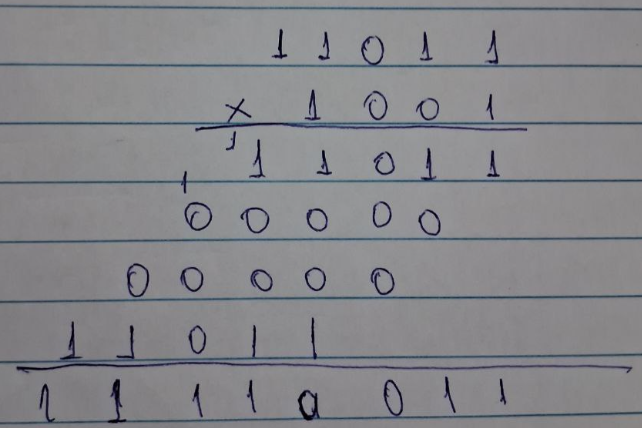
\includegraphics[width=0.7\textwidth]{Figuras/multiplicacao.png}

    \end{figure}

    \vspace{0.8cm}
    \flushleft
    \normalsize
    \textbf{Dica:} Após gerar as linhas de produto, aplique a regra da \textbf{soma binária} com atenção aos "vai um" (carries) gerados.
\end{frame}

\begin{frame}{Multiplicação Octal e Hexadecimal}
    \begin{itemize}
        \item O processo exige converter os produtos parciais para decimal e depois reconvertê-los para a base original.
        \item \textbf{Importante:} O "vai um" (carry) aqui pode ser qualquer valor, dependendo de quantas vezes a base cabe no resultado do produto.
    \end{itemize}

    \begin{exampleblock}{Exemplo Octal: $172_8 \times 30_8$}
        \centering
        \begin{tabular}{r ccccl}
                       & 1          & 7          & 2          & $_8$          &              \\
            $\times$   &            & 3          & 0          & $_8$          &              \\ \cline{2-5}
                       & 0          & 0          & 0          &               & ($\times 0$) \\
            + 5        & 5          & 6          &            &               & ($\times 3$) \\ \cline{2-5}
            \textbf{5} & \textbf{5} & \textbf{6} & \textbf{0} & \textbf{$_8$} &              \\
        \end{tabular}
    \end{exampleblock}

    \small
    \textbf{Raciocínio ($3 \times 172_8$):}
    \begin{itemize}
        \item $3 \times 2 = 6_8$.
        \item $3 \times 7 = 21_{10} \rightarrow (2 \times 8) + 5 = 25_8$. Fica \textbf{5} e vão \textbf{2}.
        \item $3 \times 1 = 3$. Com os 2 que foram: $3 + 2 = 5_8$.
    \end{itemize}
\end{frame}

\begin{frame}{Exemplo Hexadecimal: $5D2_{16} \times 51_{16}$}
    \centering
    \Large
    \begin{tabular}{r ccccc}
                   &            & 5          & D          & 2          & $_{16}$          \\
        $\times$   &            &            & 5          & 1          & $_{16}$          \\ \cline{2-6}
                   &            & 5          & D          & 2          & (x1)             \\
        + 1        & D          & 1          & A          &            & (x5)             \\ \cline{2-6}
        \textbf{1} & \textbf{D} & \textbf{7} & \textbf{7} & \textbf{2} & \textbf{$_{16}$} \\
    \end{tabular}

    \vspace{0.4cm}
    \flushleft
    \small
    \textbf{Destaque do cálculo (x5):}
    \begin{itemize}
        \item $5 \times 2 = 10_{10} = \mathbf{A_{16}}$.
        \item $5 \times D (13) = 65_{10} \rightarrow (4 \times 16) + 1 = \mathbf{41_{16}}$. Fica \textbf{1} e vão \textbf{4}.
        \item $5 \times 5 = 25_{10}$. Com o carry: $25 + 4 = 29_{10} \rightarrow (1 \times 16) + 13 = \mathbf{1D_{16}}$.
    \end{itemize}
\end{frame}

\begin{frame}{Exercícios: Multiplicação em Bases Diversas}
    Realize as operações diretamente na base indicada:

    \begin{block}{Binário e Octal}
        \begin{enumerate}[a)]
            \item $1010_2 \times 11_2$
            \item $1100_2 \times 101_2$
            \item $123_8 \times 43_8$
        \end{enumerate}
    \end{block}

    \begin{block}{Hexadecimal}
        \begin{enumerate}[d)]
            \item $1A2_{16} \times 21_{16}$
        \end{enumerate}
    \end{block}




\end{frame}

\begin{frame}{Gabarito: Multiplicação}
    \textbf{Respostas:}
    \begin{enumerate}[a)]
        \item $1010_2 \times 11_2 = $ \textcolor{red}{$11110_2$}
        \item $1100_2 \times 101_2 = $  \textcolor{red}{$111100_2$}



        \item $123_8 \times 43_8$=
              \textcolor{red}{$5531_8$}




        \item $1A2_{16} \times 21_{16}$=
              \textcolor{red}{$35E2_{16}$}
    \end{enumerate}
\end{frame}

\begin{frame}{Divisão Binária}
    \begin{itemize}
        \item O algoritmo é idêntico ao da divisão decimal (método da chave).
        \item \textbf{Vantagem:} Cada bit do quociente só pode ser \textbf{0} ou \textbf{1}.
              \begin{itemize}
                  \item \textbf{1:} Se o dividendo parcial for maior ou igual ao divisor.
                  \item \textbf{0:} Se o dividendo parcial for menor que o divisor.
              \end{itemize}
        \item É a operação base para implementações de hardware em camadas próximas ao processador.
    \end{itemize}

    \begin{exampleblock}{Exemplo: $100100_2 \div 111_2$}
        \begin{figure}[h]
            \centering
            % Substitua pelo caminho correto da sua imagem
            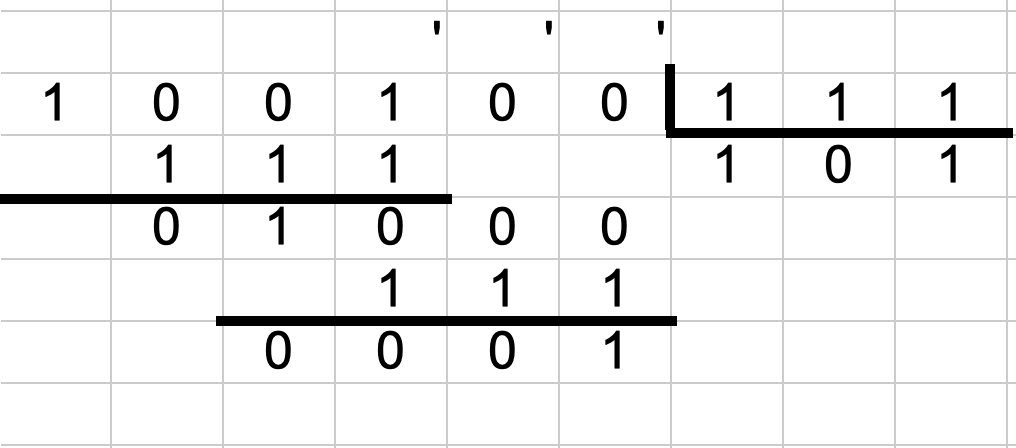
\includegraphics[width=.6\textwidth]{Figuras/divbinaria.png}
            \caption{Processo de divisão bit a bit}
            \label{fig-divbinaria}
        \end{figure}
    \end{exampleblock}
\end{frame}

\begin{frame}{Passo a Passo da Divisão: $100100_2 \div 111_2$}
    \small
    \begin{enumerate}
        \item \textbf{Busca:} Percorremos o dividendo da esquerda para a direita até encontrar um valor $\geq$ ao divisor ($111_2$).
        \item \textbf{Primeiro Bit:} Como $1001_2 \geq 111_2$, o primeiro bit do quociente é \textbf{1}.
        \item \textbf{Subtração:} $1001_2 - 111_2 = 0010_2$ (resto parcial).
        \item \textbf{Baixar Bit:} "Baixamos" o próximo $0$. O novo dividendo parcial é $100_2$.
        \item \textbf{Bit Zero:} Como $100_2 < 111_2$, o próximo bit do quociente é \textbf{0}.
        \item \textbf{Novo Bit:} Baixamos o último $0$. Agora temos $1000_2$.
        \item \textbf{Bit Um:} Como $1000_2 \geq 111_2$, o bit final do quociente é \textbf{1}.
        \item \textbf{Resto Final:} $1000_2 - 111_2 = 001_2$.
    \end{enumerate}

    \vspace{0.2cm}
    \centering
    \textbf{Resultado:} Quociente = $101_2$ | Resto = $1_2$
\end{frame}